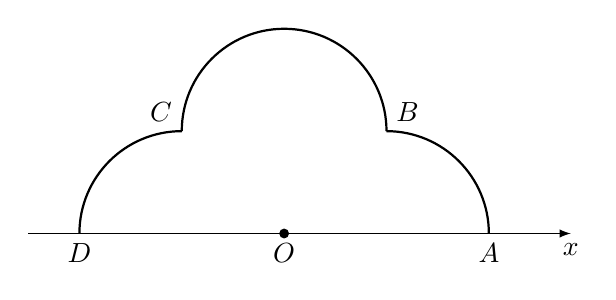
\begin{tikzpicture}[>=latex, scale=1.3]
  % 极轴
  \draw[->] (-2.5,0) -- (2.8,0) node[below] {$x$};
  
  % 原点 O
  \filldraw (0,0) circle (1.2pt) node[below] {$O$};

  % 点 D(-2, 0) 与 点 A(2, 0)
  \coordinate (D) at (-2,0);
  \coordinate (A) at (2,0);
  \node[below] at (D) {$D$};
  \node[below] at (A) {$A$};

  % 弧 AB: 圆心 (1, 0), 半径 1, 极角从 0 到 90 度 (相对于圆心: (2,0) 到 (1,1))
  % 圆心在 (1, 0), 半径 1: (1,0) + (cos t, sin t), t 从 0 到 90 度
  \draw[thick] (1,0) ++(0:1) arc (0:90:1);
  \coordinate (B) at (1,1);
  \node[above right] at (B) {$B$};

  % 弧 BC: 圆心 (0, 1), 半径 1: (0,1) + (cos t, sin t), 从 B(1, 1) 即 t=0 到 (0, 2) 即 t=90 到 C(-1, 1) 即 t=180
  \draw[thick] (0,1) ++(0:1) arc (0:180:1);
  \coordinate (C) at (-1,1);
  \node[above left] at (C) {$C$};

  % 弧 CD: 圆心 (-1, 0), 半径 1: 从 C(-1, 1) 即相对于圆心 (-1, 0) 为 90 度到 180 度即 (-2, 0)
  \draw[thick] (-1,0) ++(90:1) arc (90:180:1);
\end{tikzpicture}